\chapter{Supplementary Material for Chapter~\ref{ch:occnet}}\label{app:occnet}

This appendix collects material that supports Chapter~\ref{ch:occnet}: the evaluation metrics (Section~\ref{occnet:app:metrics}), implementation details of OccNet and of the BEVNet and VoxelNet baselines (Section~\ref{occnet:app:implementation}), details and statistics of the OpenOcc benchmark (Section~\ref{occnet:app:openocc}), additional experiments (Section~\ref{occnet:app:experiments}), and further visualisations (Section~\ref{occnet:app:visualization}).

%-----------------------------------------------------------------------
\section{Evaluation Metrics}\label{occnet:app:metrics}

\paragraph{Semantic scene completion.} For scene completion, the model predicts the semantic label of each voxel in 3D space. The evaluation metric is the mean intersection-over-union (mIoU) over all classes,
\begin{equation}
  \text{mIoU} = \frac{1}{C}\sum_{c=1}^{C}\frac{\text{TP}_c}{\text{TP}_c+\text{FP}_c+\text{FN}_c},
  \label{occnet:eq:miou}
\end{equation}
where $C=16$ is the number of classes in the benchmark, and $\text{TP}_c$, $\text{FP}_c$ and $\text{FN}_c$ are the true positive, false positive and false negative predictions for class $c$, respectively. In addition, the class-agnostic metric $\text{IoU}_{\text{geo}}$ evaluates the quality of the geometric reconstruction of the scene.

\paragraph{3D object detection.} Detection is evaluated with the official nuScenes metrics~\cite{caesar2020nuscenes}, namely the nuScenes detection score (NDS), mean average precision (mAP), average translation error (ATE), average scale error (ASE), average orientation error (AOE), average velocity error (AVE) and average attribute error (AAE).

\paragraph{Motion planning.} For planning, we follow the metrics of ST-P3~\cite{hu2022stp3}. The L2 distance between the planned trajectory and the ground-truth trajectory measures the regression accuracy, and the collision rate with other vehicles and pedestrians measures the safety of the future actions.

%-----------------------------------------------------------------------
\section{Implementation Details of OccNet}\label{occnet:app:implementation}

\paragraph{Backbone and multi-scale features.} Following previous work~\cite{li2022bevformer,wang2021fcos3d}, we adopt ResNet101~\cite{he2016deep} as the backbone, with an FPN~\cite{lin2017feature} to extract multi-scale features from the multi-view images. We use the output features of stages $S_3$, $S_4$ and $S_5$ of ResNet101, where $S_n$ has a downsampling factor of $1/2^n$ and a feature dimension of $C_n=256\times2^{n-2}$. The FPN aggregates these features and transforms them into three levels with sizes of 1/16, 1/32 and 1/64 and a dimension of 256.

\paragraph{BEV encoder.} The BEV encoder follows the structure of BEVFormer~\cite{li2022bevformer} and transforms the multi-scale features of the FPN into the BEV feature. It comprises two encoder layers with temporal self-attention and spatial cross-attention, through which the BEV query $Q_t$ is refined progressively by the spatial-temporal transformer mechanism to learn a scene representation in BEV space.

\paragraph{Feature transformation in the voxel decoder.} To lift the voxel feature $V'_{t,i}\in\mathbb{R}^{Z_i\times H\times W\times C_i}$ to $V'_{t,i+1}\in\mathbb{R}^{Z_{i+1}\times H\times W\times C_{i+1}}$, an MLP transforms the feature dimension from $Z_i\times C_i$ to $Z_{i+1}\times C_{i+1}$. For the spatial cross-attention of $V'_{t,i}$, the multi-scale image features of the FPN, whose dimension is 256, are transformed to dimension $C_i$ by an MLP.

\paragraph{Training strategy.} Following previous work~\cite{li2022bevformer,wang2021fcos3d}, we train OccNet for 24 epochs with a learning rate of $2\times10^{-4}$, a batch size of one sample (six images) per GPU, and the AdamW optimiser~\cite{loshchilov2017decoupled} with a weight decay of $1\times10^{-2}$. For the downstream tasks, all perception tasks except BEV segmentation are trained at once, and the other tasks are fine-tuned on top of the frozen tasks.

\paragraph{VoxelNet and BEVNet.} Unlike OccNet, whose feature maps are cascaded, VoxelNet and BEVNet use a single-scale feature map. VoxelNet uses voxel queries $Q_{\text{voxel}}\in\mathbb{R}^{4\times H\times W}$ to construct the voxel feature map $F_{\text{voxel}}\in\mathbb{R}^{4\times H\times W\times C_1}$ directly from the image features with 3D-DA (Eq.~\eqref{occnet:eq:3dda}), and expands it to the full-scale occupancy $V\in\mathbb{R}^{16\times H\times W\times C_2}$ with a fully connected layer. BEVNet generates a BEV feature $F_{\text{bev}}\in\mathbb{R}^{H\times W\times C_1}$ as in BEVFormer and reshapes it directly to the voxel feature $V\in\mathbb{R}^{16\times H\times W\times C_2}$. Here $C_1$ and $C_2$ denote numbers of channels. Both VoxelNet and BEVNet also adopt temporal context fusion.

%-----------------------------------------------------------------------
\section{More Details about OpenOcc}\label{occnet:app:openocc}

\begin{figure}[t]
  \centering
  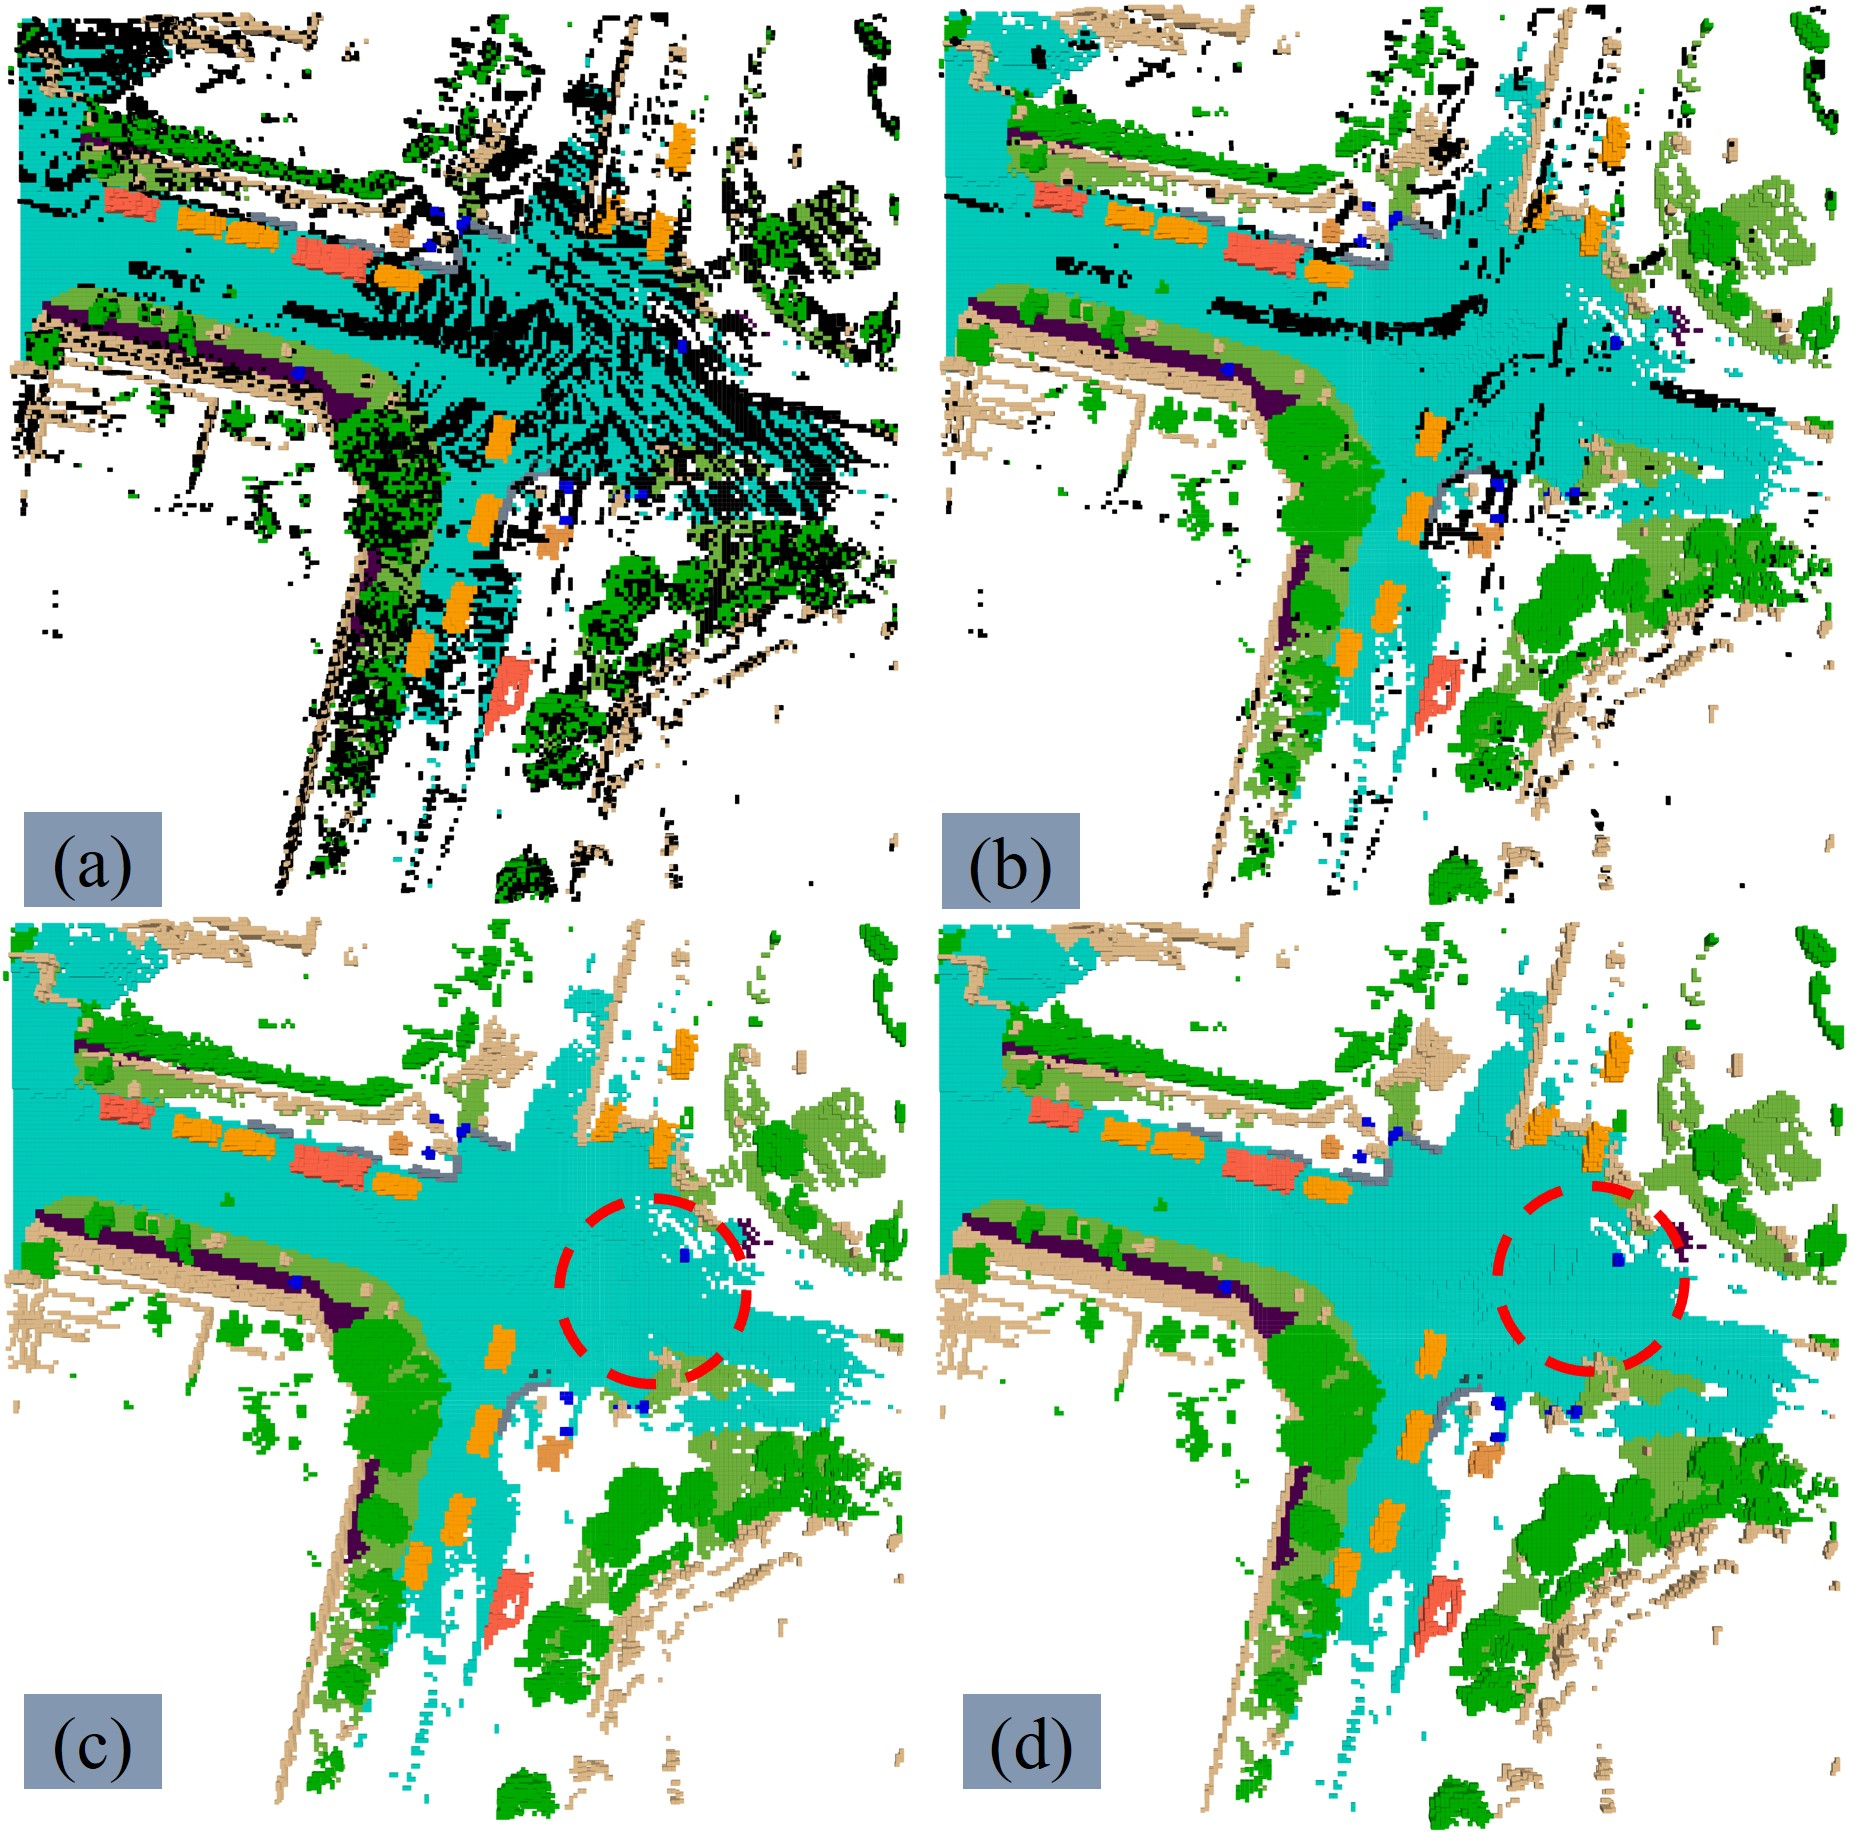
\includegraphics[width=0.72\linewidth]{ch-occnet/images/fig_occ_gt_pipeline_used.jpg}
  \caption[Generation of the OpenOcc annotations]{\textbf{Generation of the OpenOcc annotations.} (a)~Occupancy generated from object points and partially labelled background points; black points denote unknown background points from intermediate frames. (b)~Part of the unknown background points is annotated from the generated occupancy. (c)~The remaining unknown background points are removed as noise. (d)~Post-processing ensures the completeness of the scene, \eg by filling holes (red dashed box).}
  \label{occnet:fig:occ_gt_pipeline}
\end{figure}

\paragraph{Accumulation of foreground objects.} To accumulate the foreground objects, we split the LiDAR points into object points and background points. The nuScenes dataset~\cite{caesar2020nuscenes}, however, does not provide 3D box annotations for intermediate frames. We approximate these boxes by linear interpolation between the two adjacent key frames, which allows us to accumulate dense object points from the available intermediate LiDAR points.

\paragraph{Dataset generation pipeline.} With the accumulated dense background points and foreground object points, we generate the occupancy data following the pipeline shown in Fig.~\ref{occnet:fig:occ_gt_pipeline}. The occupancy data are refined step by step into the dense and high-quality annotations of Fig.~\ref{occnet:fig:occ_gt_pipeline}(d).

\paragraph{Dataset statistics.} We annotate 16 classes in 34,149 frames for all 700 training and 150 validation scenes, with over 1.4 billion voxels. Fig.~\ref{occnet:fig:statistics_occ} shows the label distribution of the 16 classes, which indicates a great diversity in the benchmark. The dataset exhibits a significant class imbalance: the 10 foreground classes account for only 5.33\% of all labels, and bicycle and motorcycle for only 0.02\% and 0.03\%, respectively. We additionally provide flow annotations for eight foreground classes, which help downstream tasks such as motion planning. We split objects into a moving and a stationary state with a velocity threshold of $v_{\text{th}}=0.2$\,m/s; Fig.~\ref{occnet:fig:statistics_flow} gives the percentage of moving objects for each class. More than 50\% of the foreground objects are moving, which underlines the significance of motion information in driving scenes.

\begin{figure}[t]
  \centering
  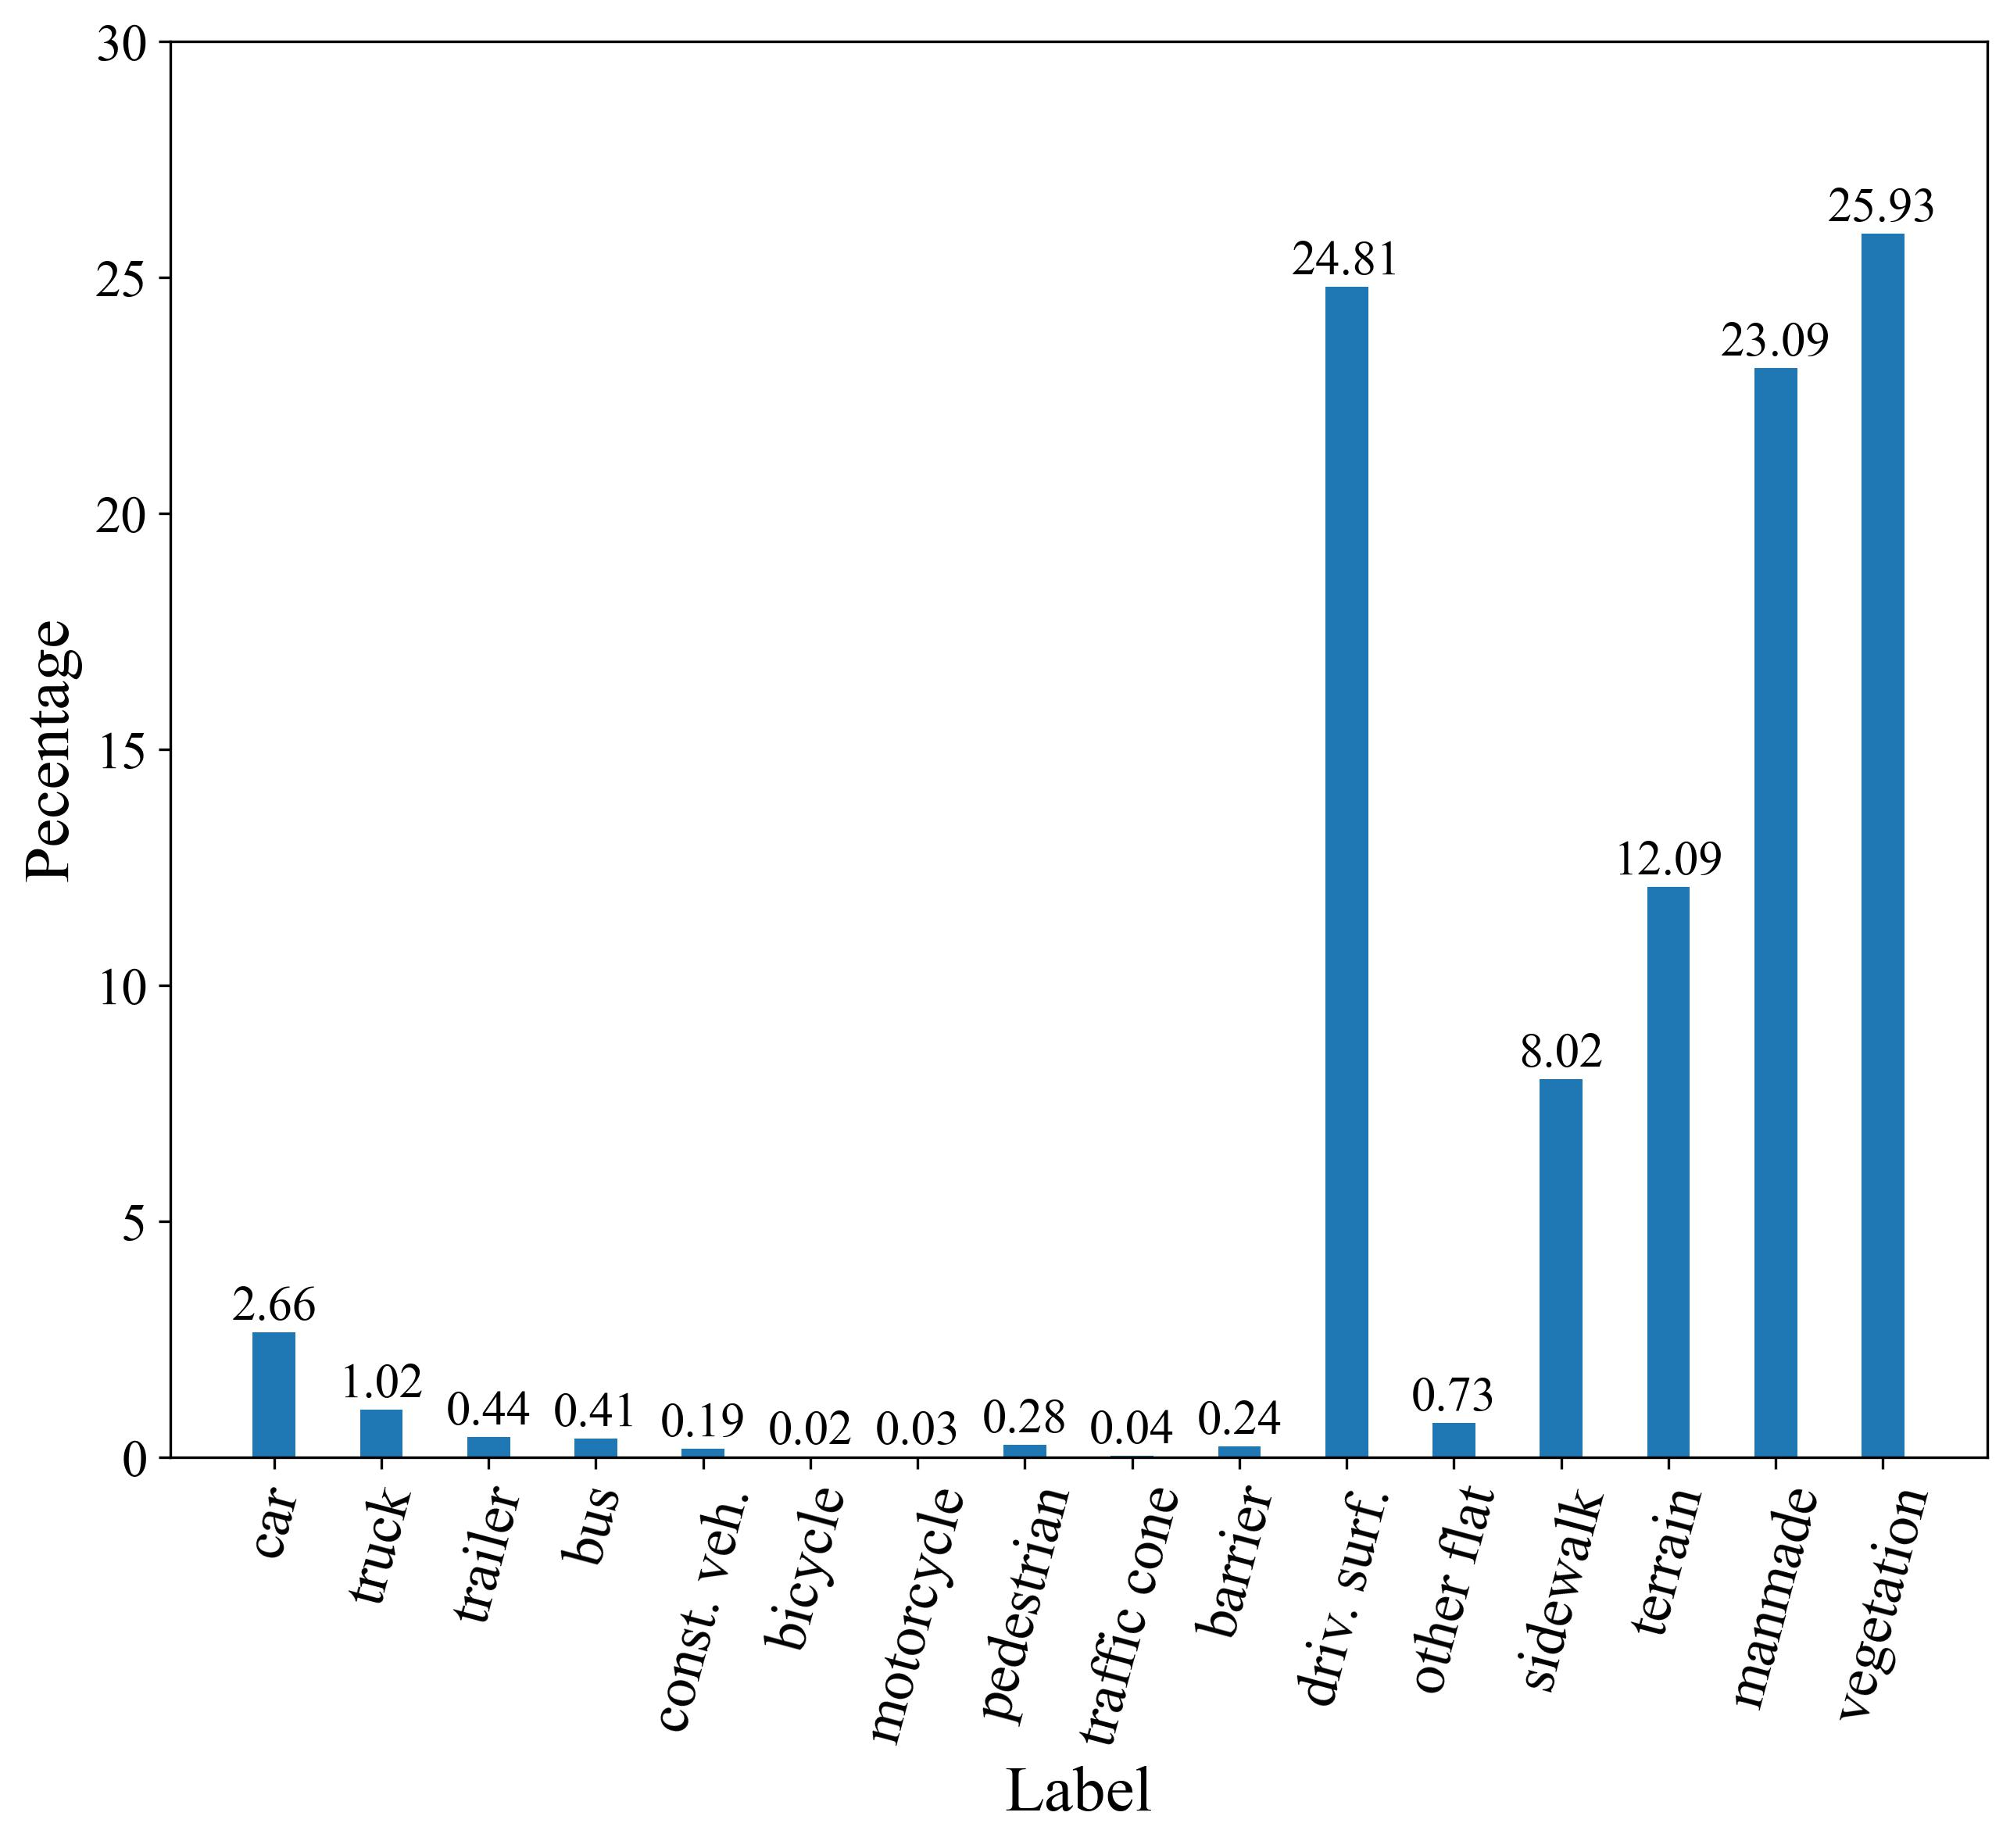
\includegraphics[width=0.66\linewidth]{ch-occnet/images/fig_occ_label_distribution_used.jpg}
  \caption[Distribution of occupancy classes in OpenOcc]{\textbf{Distribution of occupancy classes in the OpenOcc benchmark.} Background stuff forms the majority of the occupancy labels.}
  \label{occnet:fig:statistics_occ}
\end{figure}

\begin{figure}[t]
  \centering
  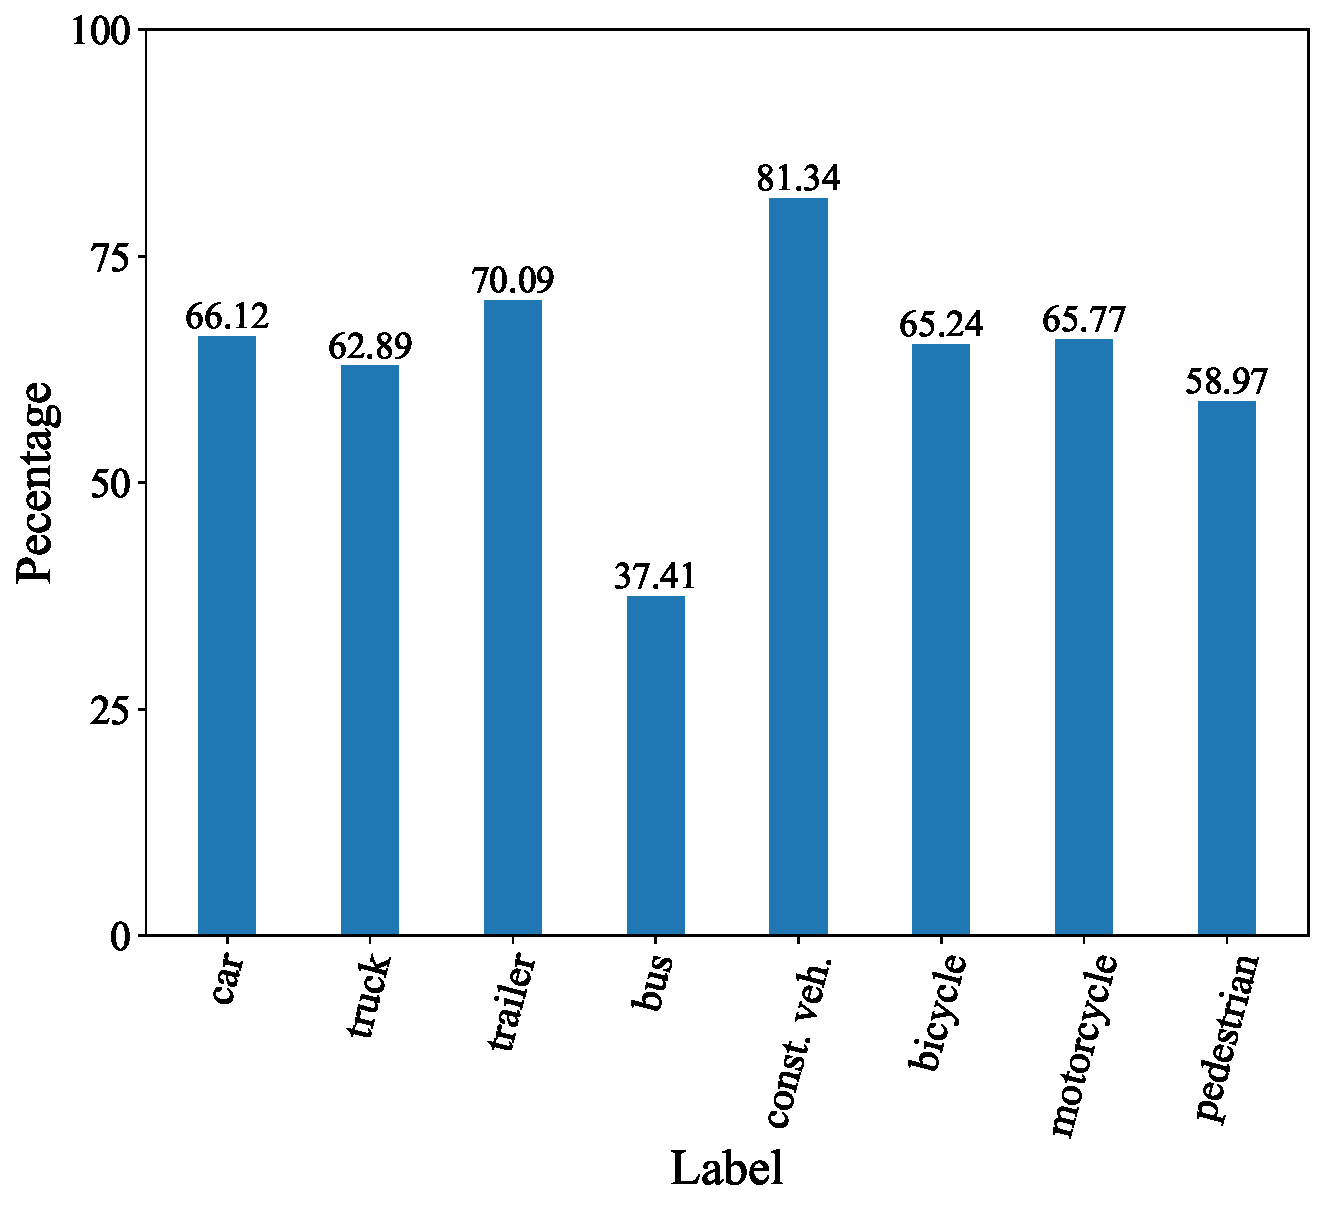
\includegraphics[width=0.72\linewidth]{ch-occnet/images/fig_flow_distribution_used.pdf}
  \caption[Percentage of moving occupancy for each foreground class]{\textbf{Percentage of occupancy with velocity for each foreground class.} Of the 10 foreground classes in the benchmark, only the 8 movable classes are considered.}
  \label{occnet:fig:statistics_flow}
\end{figure}

%-----------------------------------------------------------------------
\section{Additional Experiments}\label{occnet:app:experiments}

\paragraph{Number of frames for temporal self-attention.} We investigate the effect of the number of frames used by the temporal self-attention during training. Tables~\ref{occnet:tab:frame_number_ssc} and~\ref{occnet:tab:frame_number_lidarseg} show that adding temporal frames improves performance, and that the improvement slows down once a threshold of four frames is reached. Too few history frames, however, hurt performance to some extent: with a single history frame, both tasks are worse than without temporal context (18.35 \vs 19.21 mIoU on scene completion and 48.41 \vs 53.82 mIoU on LiDAR segmentation).

\begin{table}[t]
  \centering
  \caption[Effect of history frames on semantic scene completion]{\textbf{Effect of the number of history frames on semantic scene completion} (OccNet, ResNet50). \#Num: number of history frames used in training. $^{\ast}$: setting used in the main experiments.}
  \label{occnet:tab:frame_number_ssc}
  \begin{tabular}{lccccc}
    \toprule
    \#Num & $\text{IoU}_{\text{geo}}$$\uparrow$ & mIoU$\uparrow$ & Barrier$\uparrow$ & Bicycle$\uparrow$ & Bus$\uparrow$ \\
    \midrule
    0          & 37.49 & 19.21 & 20.07 & 4.70 & 24.11 \\
    1          & 36.89 & 18.35 & 18.77 & 4.51 & 21.66 \\
    2$^{\ast}$ & 37.69 & 19.48 & 20.63 & 5.52 & 24.16 \\
    3          & 38.36 & 20.30 & 21.39 & 6.47 & 24.65 \\
    4          & 39.21 & \textbf{20.81} & \textbf{22.30} & 5.66 & \textbf{25.13} \\
    9          & \textbf{39.36} & 20.68 & 20.75 & \textbf{7.83} & 24.79 \\
    \bottomrule
  \end{tabular}
\end{table}

\begin{table}[t]
  \centering
  \caption[Effect of history frames on LiDAR segmentation]{\textbf{Effect of the number of history frames on LiDAR segmentation} (OccNet, ResNet50). \#Num: number of history frames used in training.}
  \label{occnet:tab:frame_number_lidarseg}
  \begin{tabular}{lcccccc}
    \toprule
    \#Num & mIoU$\uparrow$ & Barrier$\uparrow$ & Bicycle$\uparrow$ & Bus$\uparrow$ & Car$\uparrow$ & Truck$\uparrow$ \\
    \midrule
    0 & 53.82 & 59.02 & 24.05 & 67.61 & 69.59 & 59.38 \\
    1 & 48.41 & 57.45 & 21.52 & 57.71 & 67.26 & 44.60 \\
    2 & 52.33 & 61.41 & 26.07 & 73.97 & 70.56 & 52.64 \\
    3 & 53.49 & 60.98 & 24.45 & 70.20 & 69.37 & 56.84 \\
    4 & \textbf{54.59} & \textbf{62.09} & 21.06 & 75.05 & 70.20 & 59.40 \\
    9 & 54.35 & 60.04 & \textbf{30.83} & \textbf{75.49} & \textbf{71.02} & \textbf{61.63} \\
    \bottomrule
  \end{tabular}
\end{table}

\paragraph{Evaluating planning with occupancy-based collisions.} Instead of the bounding boxes of vehicles and pedestrians, we use the ground-truth occupancy to evaluate the planner. Specifically, the collision rate is computed between the trajectory and all foreground occupancy voxels plus the voxels of four background classes, \ie other flat, terrain, manmade and vegetation. As Table~\ref{occnet:tab:occupancy_metrics} shows, occupancy input for the planning model remains advantageous in most intervals under this metric. In future research, a cost function designed specifically for occupancy input may further improve planning.

\begin{table}[t]
  \centering
  \caption[Planning evaluated with occupancy-based collisions]{\textbf{Planning results with different scene representations under the occupancy-based collision metric.} Occupancy input remains advantageous in most intervals.}
  \label{occnet:tab:occupancy_metrics}
  \begin{tabular}{lcccccc}
    \toprule
    \multirow{2}{*}{Input} & \multicolumn{3}{c}{Collision (\%)$\downarrow$} & \multicolumn{3}{c}{L2 (m)$\downarrow$} \\
    \cmidrule(lr){2-4}\cmidrule(lr){5-7}
     & 1\,s & 2\,s & 3\,s & 1\,s & 2\,s & 3\,s \\
    \midrule
    Bbox GT      & 1.66 & 2.88 & 4.37 & 1.33 & 2.18 & 3.03 \\
    Occupancy GT & \textbf{1.63} & \textbf{2.85} & \textbf{4.29} & \textbf{1.29} & \textbf{2.13} & \textbf{2.99} \\
    \midrule
    Bbox pred.\ (OccNet)      & 1.75 & \textbf{2.85} & 4.37 & 1.33 & 2.17 & 3.04 \\
    \rowcolor{perceive!10} Occupancy pred.\ (OccNet) & \textbf{1.68} & 2.94 & \textbf{4.32} & \textbf{1.30} & \textbf{2.15} & \textbf{3.02} \\
    \bottomrule
  \end{tabular}
\end{table}

\paragraph{Pre-training for planning.} Having evaluated pre-trained models on 3D detection and BEV segmentation in Section~\ref{occnet:sec:main_results}, we further examine their effect on the downstream planning task. Specifically, we replace the perception module of ST-P3~\cite{hu2022stp3} with a pre-trained OccNet and fine-tune the planning module. Unfortunately, pre-training on occupancy does not provide an advantage for planning (Table~\ref{occnet:tab:planning_pretrain}). Combined with the planning experiment of Section~\ref{occnet:sec:main_results}, this indicates that the planning task should directly use the scene completion results of occupancy rather than the pre-trained features.

\begin{table}[t]
  \centering
  \caption[Pre-training tasks for planning]{\textbf{Pre-training tasks for planning.} Features pre-trained on occupancy do not directly benefit planning.}
  \label{occnet:tab:planning_pretrain}
  \begin{tabular}{lcccccc}
    \toprule
    \multirow{2}{*}{Pre-training} & \multicolumn{3}{c}{Collision (\%)$\downarrow$} & \multicolumn{3}{c}{L2 (m)$\downarrow$} \\
    \cmidrule(lr){2-4}\cmidrule(lr){5-7}
     & 1\,s & 2\,s & 3\,s & 1\,s & 2\,s & 3\,s \\
    \midrule
    Det & \textbf{0.38} & \textbf{0.40} & \textbf{0.82} & \textbf{0.85} & \textbf{1.18} & \textbf{1.57} \\
    Occ & 0.47 & 0.68 & 1.03 & 0.93 & 1.26 & 1.70 \\
    \bottomrule
  \end{tabular}
\end{table}

\paragraph{Decoder ablation on semantic scene completion.} Table~\ref{occnet:tab:occ_ablation} compares BEVNet, VoxelNet and OccNet on semantic scene completion per class. The cascaded voxel structure helps learn a better occupancy descriptor of 3D space with both backbones.

\begin{table}[t]
  \centering
  \caption[Decoder ablation on semantic scene completion]{\textbf{Ablation of the decoder design on semantic scene completion.} OccNet outperforms BEVNet and VoxelNet.}
  \label{occnet:tab:occ_ablation}
  \setlength{\tabcolsep}{3.5pt}
  \resizebox{\textwidth}{!}{%
  \begin{tabular}{@{}llcc*{16}{c}@{}}
    \toprule
    Method & Backbone & $\text{IoU}_{\text{geo}}$ & mIoU & \rotatebox{90}{barrier} & \rotatebox{90}{bicycle} & \rotatebox{90}{bus} & \rotatebox{90}{car} & \rotatebox{90}{const.\ veh.} & \rotatebox{90}{motorcycle} & \rotatebox{90}{pedestrian} & \rotatebox{90}{traffic cone} & \rotatebox{90}{trailer} & \rotatebox{90}{truck} & \rotatebox{90}{driv.\ surf.} & \rotatebox{90}{other flat} & \rotatebox{90}{sidewalk} & \rotatebox{90}{terrain} & \rotatebox{90}{manmade} & \rotatebox{90}{vegetation} \\
    \midrule
    BEVNet   & ResNet50 & 36.11 & 17.37 & 14.02 & 5.07 & 20.85 & 24.94 & 8.64 & 7.75 & 12.8 & 8.93 & 10.21 & 16.02 & 44.41 & 14.42 & 23.87 & 27.76 & 13.73 & 24.49 \\
    VoxelNet & ResNet50 & 37.59 & 19.06 & 19.31 & 6.25 & 22.16 & 26.89 & 9.96 & 6.91 & 12.70 & 6.27 & 9.43 & 16.96 & 46.7 & 23.31 & 26.04 & 29.08 & 16.52 & 26.46 \\
    \rowcolor{perceive!10} OccNet & ResNet50 & 37.69 & 19.48 & 20.63 & 5.52 & 24.16 & 27.72 & 9.79 & 7.73 & 13.38 & 7.18 & 10.68 & 18.00 & 46.13 & 20.60 & 26.75 & 29.37 & 16.90 & 27.21 \\
    \midrule
    BEVNet   & ResNet101 & 40.15 & 24.62 & 26.39 & 15.79 & 32.07 & 35.83 & 11.93 & 19.72 & 19.75 & 15.38 & 12.82 & 23.90 & 49.16 & 21.52 & 30.57 & 31.39 & 18.99 & 28.71 \\
    VoxelNet & ResNet101 & 40.73 & 26.06 & 27.98 & 15.95 & 32.31 & 36.15 & 14.88 & 20.55 & 20.72 & 16.52 & 15.13 & 25.94 & 49.07 & 27.82 & 31.04 & 32.43 & 20.45 & 29.99 \\
    \rowcolor{perceive!10} OccNet & ResNet101 & \textbf{41.08} & \textbf{26.98} & \textbf{29.77} & \textbf{16.89} & \textbf{34.16} & \textbf{37.35} & \textbf{15.58} & \textbf{21.92} & \textbf{21.29} & \textbf{16.75} & \textbf{16.37} & \textbf{26.23} & \textbf{50.74} & \textbf{27.93} & \textbf{31.98} & \textbf{33.24} & \textbf{20.8} & \textbf{30.68} \\
    \bottomrule
  \end{tabular}}
\end{table}

\paragraph{Effect of voxel resolution on LiDAR segmentation.} We voxelise the 3D space at resolutions $\Delta s\in\{1.0\,\text{m},0.5\,\text{m},0.25\,\text{m}\}$ to investigate the effect of voxel resolution on LiDAR segmentation. Since the semantic occupancy prediction is transferred to LiDAR segmentation by assigning each point the label of its voxel, LiDAR segmentation improves as $\Delta s$ decreases (Table~\ref{occnet:tab:lidarseg_resolution}), from 46.60 to 53.00 mIoU. This suggests that a camera-based OccNet can approach the performance of LiDAR-based methods as $\Delta s\to0$.

\begin{table}[t]
  \centering
  \caption[Effect of voxel resolution on LiDAR segmentation]{\textbf{Effect of voxel resolution on LiDAR segmentation} with OccNet (ResNet50) on the nuScenes validation set. The smallest voxel size $\Delta s$ performs best.}
  \label{occnet:tab:lidarseg_resolution}
  \setlength{\tabcolsep}{3.5pt}
  \resizebox{\textwidth}{!}{%
  \begin{tabular}{@{}lcc*{16}{c}@{}}
    \toprule
    Method & $\Delta s$ (m) & mIoU & \rotatebox{90}{barrier} & \rotatebox{90}{bicycle} & \rotatebox{90}{bus} & \rotatebox{90}{car} & \rotatebox{90}{const.\ veh.} & \rotatebox{90}{motorcycle} & \rotatebox{90}{pedestrian} & \rotatebox{90}{traffic cone} & \rotatebox{90}{trailer} & \rotatebox{90}{truck} & \rotatebox{90}{driv.\ surf.} & \rotatebox{90}{other flat} & \rotatebox{90}{sidewalk} & \rotatebox{90}{terrain} & \rotatebox{90}{manmade} & \rotatebox{90}{vegetation} \\
    \midrule
    OccNet & 1.00 & 46.60 & 52.78 & 21.04 & 65.94 & 62.45 & 18.31 & 15.49 & 30.71 & 15.82 & 33.94 & 50.22 & 83.93 & 48.84 & 50.52 & 57.89 & 69.49 & 68.29 \\
    OccNet & 0.50 & 47.29 & 59.06 & 20.63 & 48.32 & 63.05 & 24.12 & 20.24 & 41.82 & 18.84 & 23.38 & 41.12 & 86.46 & 53.12 & 52.03 & 59.14 & 71.55 & 73.68 \\
    \rowcolor{perceive!10} OccNet & 0.25 & 53.00 & 65.93 & 22.84 & 64.09 & 72.69 & 32.73 & 28.73 & 52.21 & 17.64 & 22.05 & 51.26 & 89.05 & 57.41 & 58.06 & 64.30 & 75.09 & 73.92 \\
    \bottomrule
  \end{tabular}}
\end{table}

%-----------------------------------------------------------------------
\section{Visualisation Results}\label{occnet:app:visualization}

We sample two scenes from the validation set and visualise the occupancy predictions of OccNet in detail in Fig.~\ref{occnet:fig:occ_pred}; OccNet describes the scene geometry and semantics in detail. Fig.~\ref{occnet:fig:planning2} compares rasterised occupancy with rasterised bounding boxes as the input of the planning module: with occupancy input, the planned trajectory keeps a greater safety distance from a truck.

\begin{figure}[t]
  \centering
  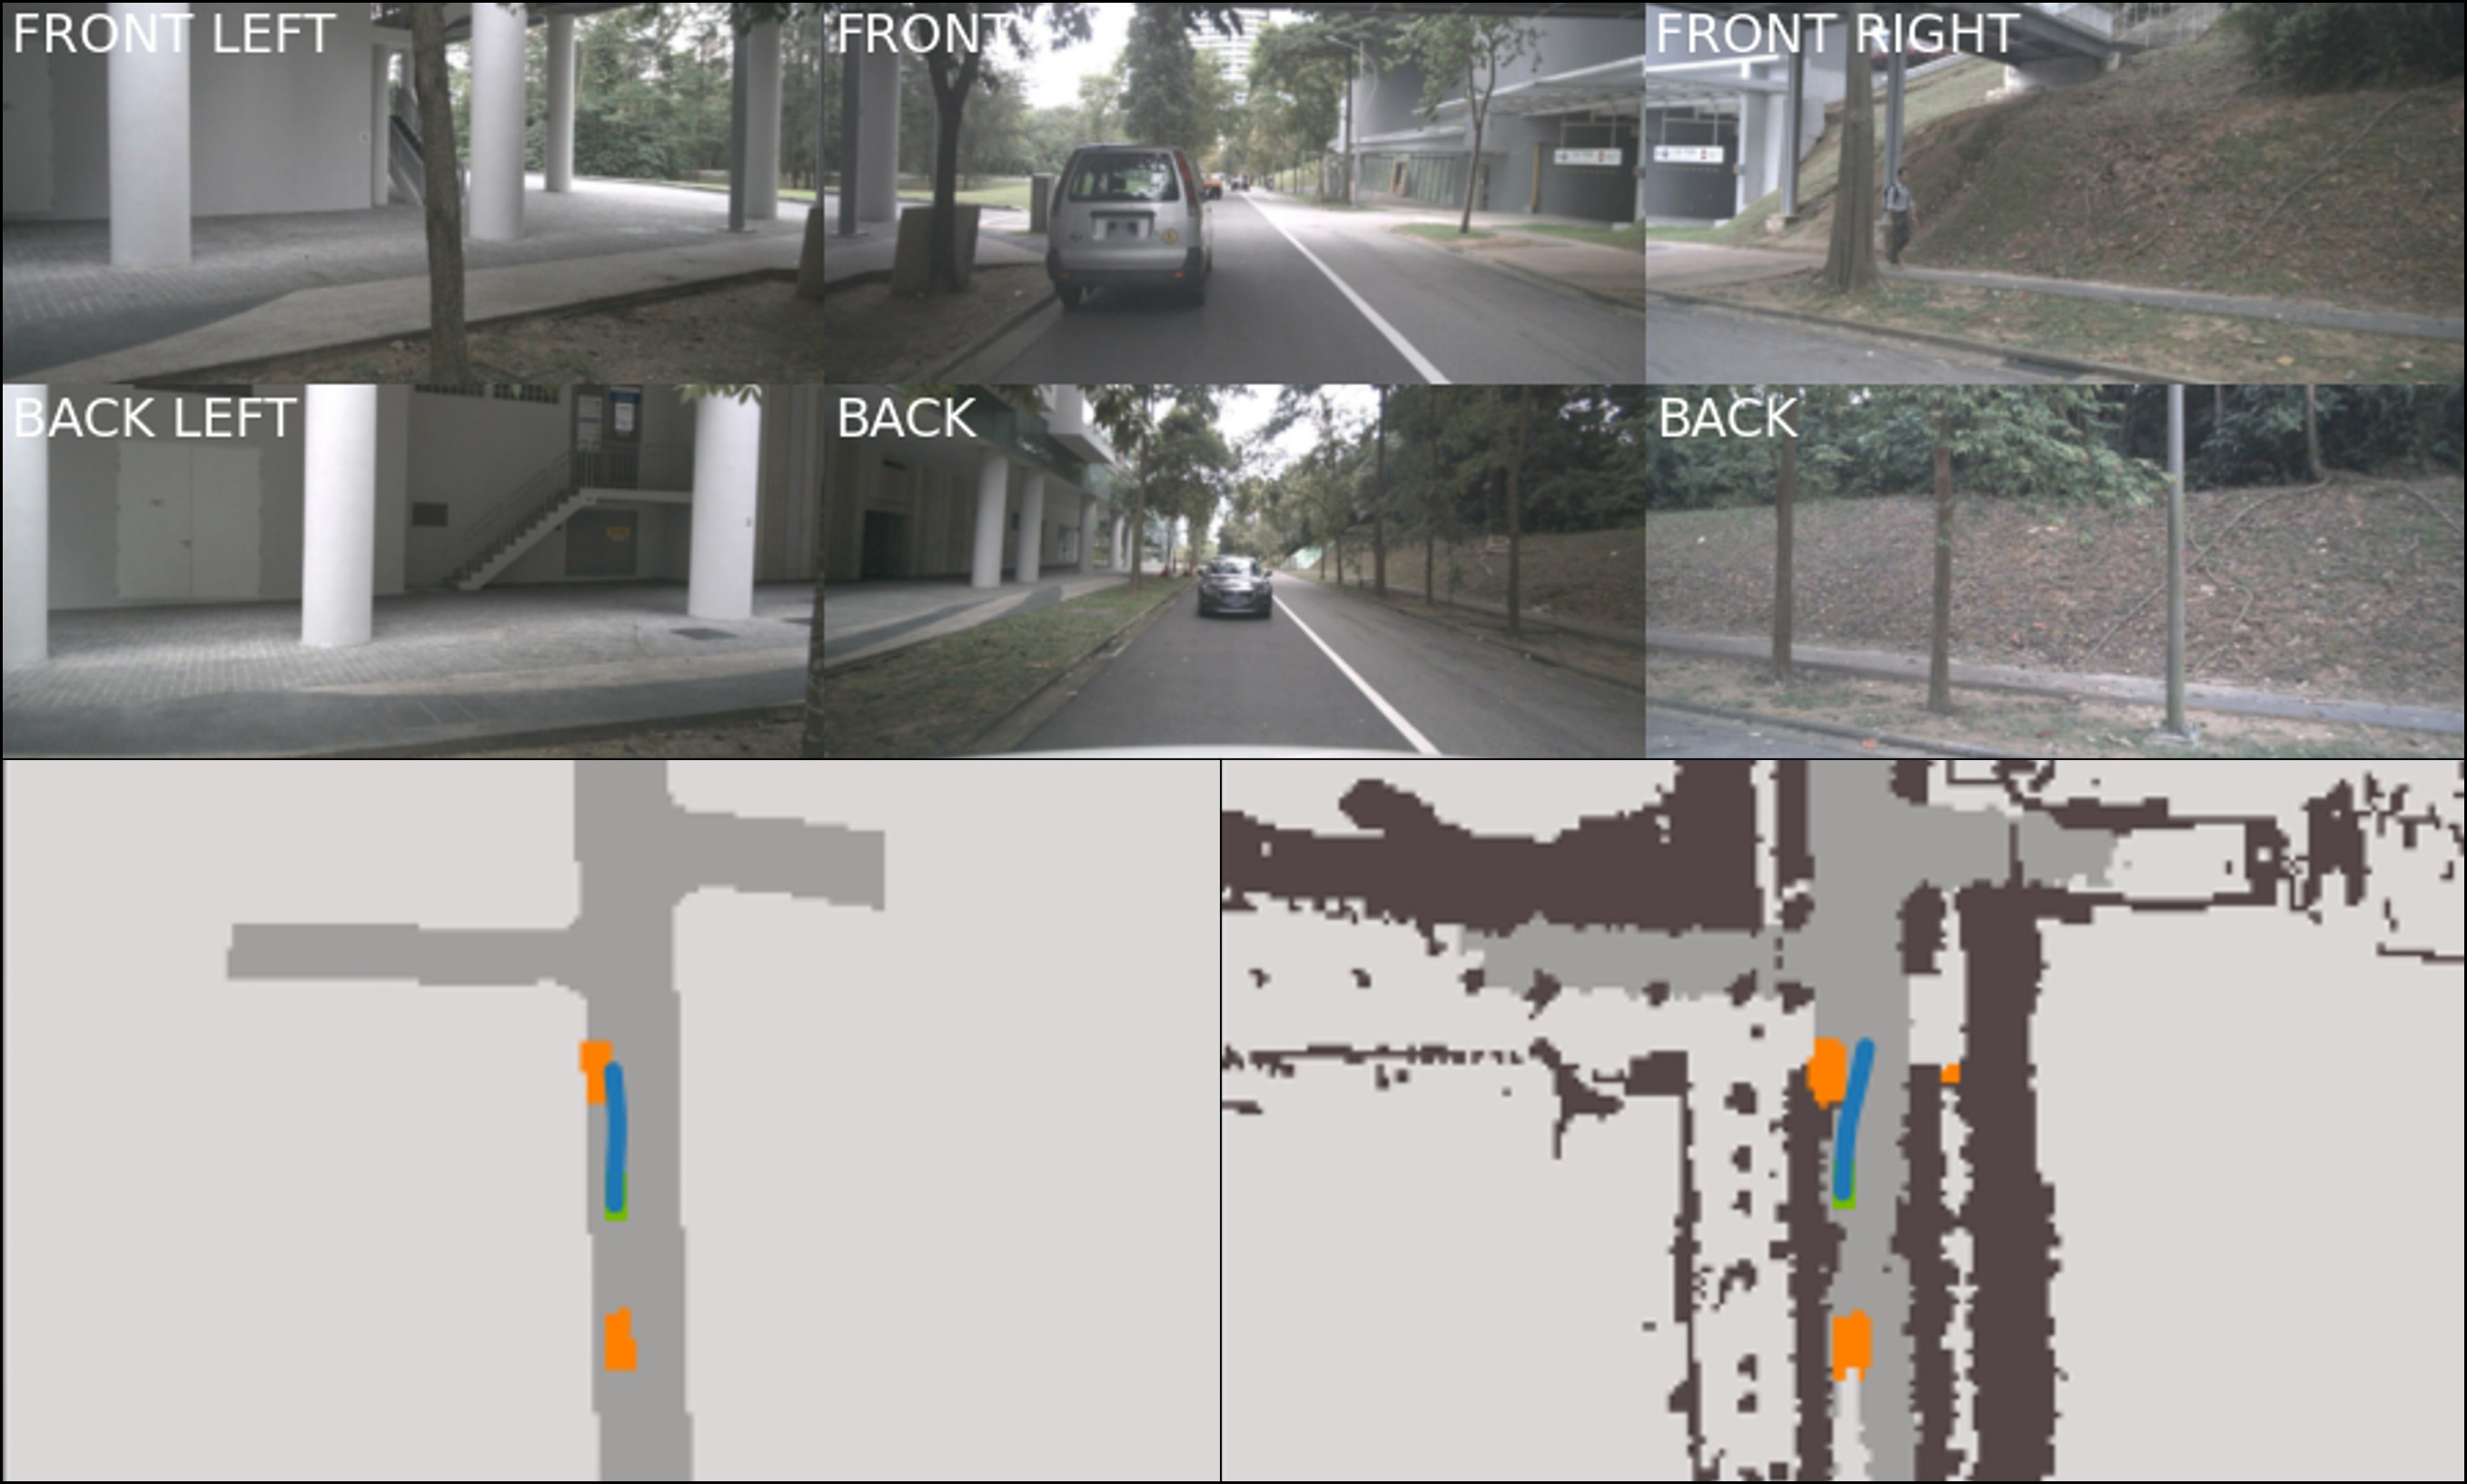
\includegraphics[width=0.86\linewidth]{ch-occnet/images/fig_planning2_used.jpg}
  \caption[Further visualisation of planning with boxes and occupancy]{\textbf{Visualisation of planning.} The blue line is the planned trajectory. The lower panels show the rasterised bounding boxes (left) and the rasterised occupancy (right) used as planning input. The trajectory obtained with rasterised occupancy keeps a greater safety distance from the truck, because occupancy represents its polygon more accurately.}
  \label{occnet:fig:planning2}
\end{figure}

\begin{figure}[t]
  \centering
  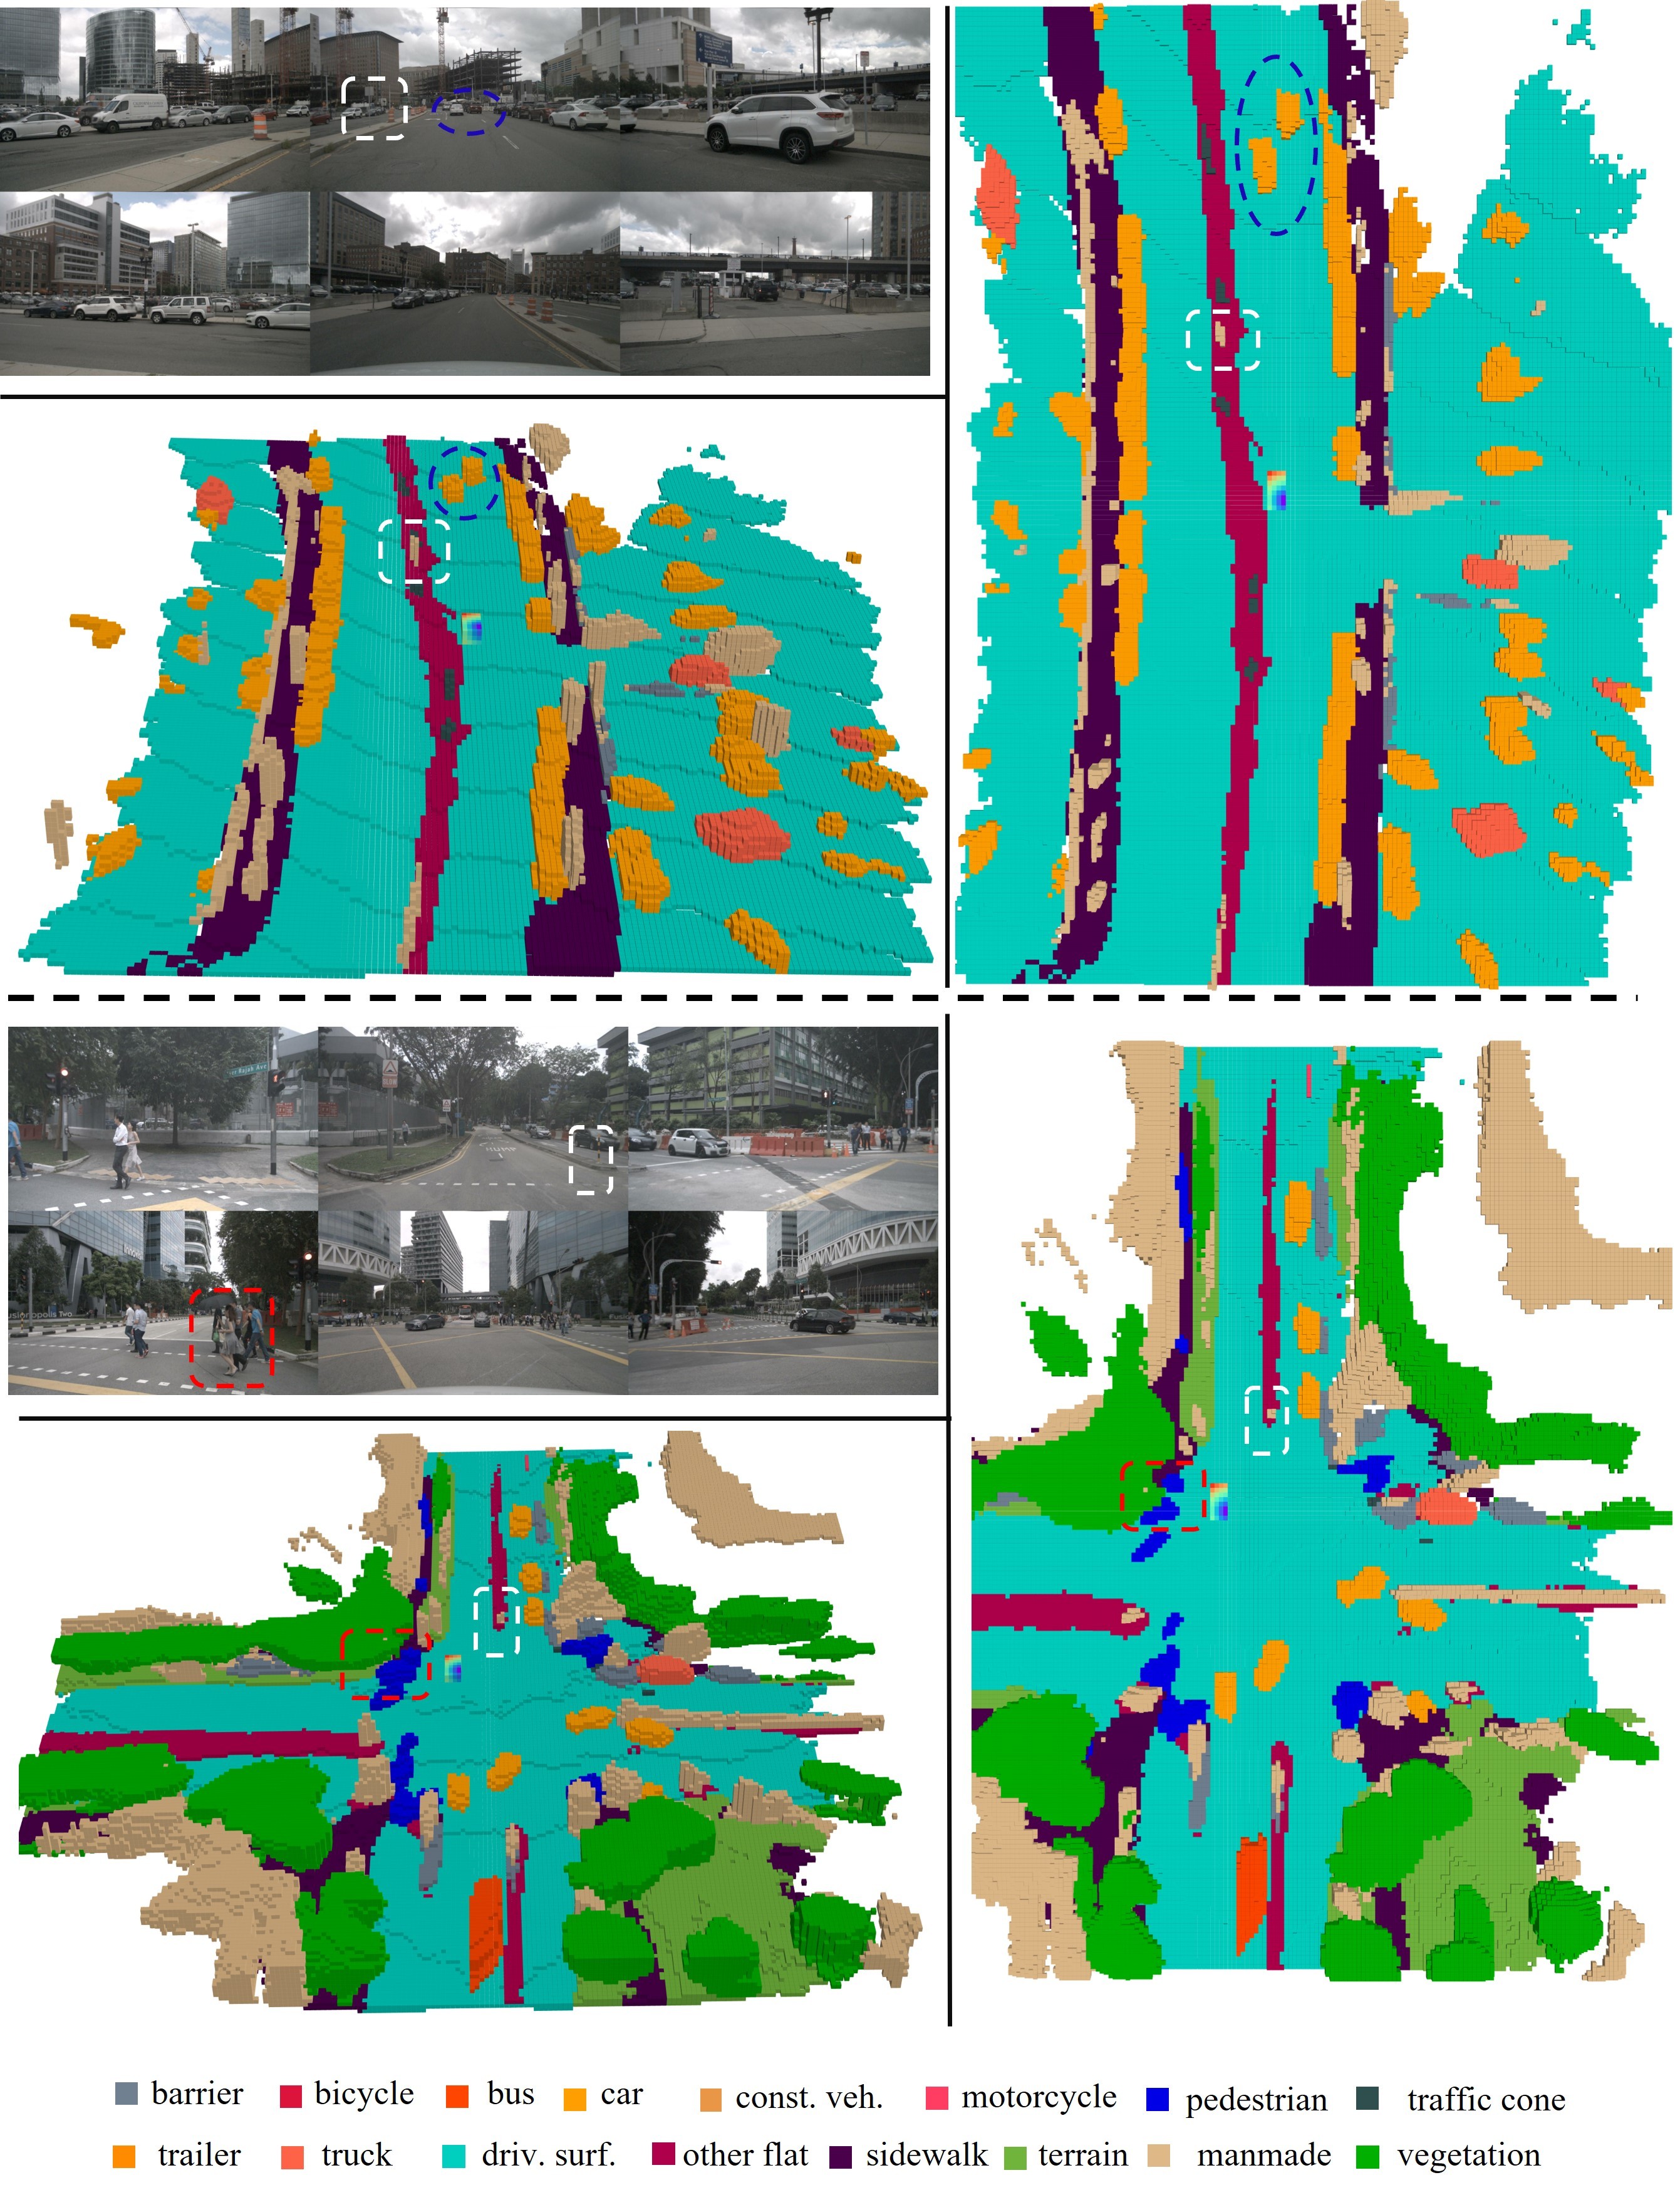
\includegraphics[width=0.8\linewidth]{ch-occnet/images/fig_occ_vis_1_used.jpg}
  \caption[Visualisation of occupancy prediction]{\textbf{Visualisation of occupancy prediction.} For each scene, the top-left panel shows the surround-view camera input, and the bottom-left and right panels show the perspective view and the top view of the predicted occupancy. The dashed regions show that OccNet predicts small or distant targets well.}
  \label{occnet:fig:occ_pred}
\end{figure}
